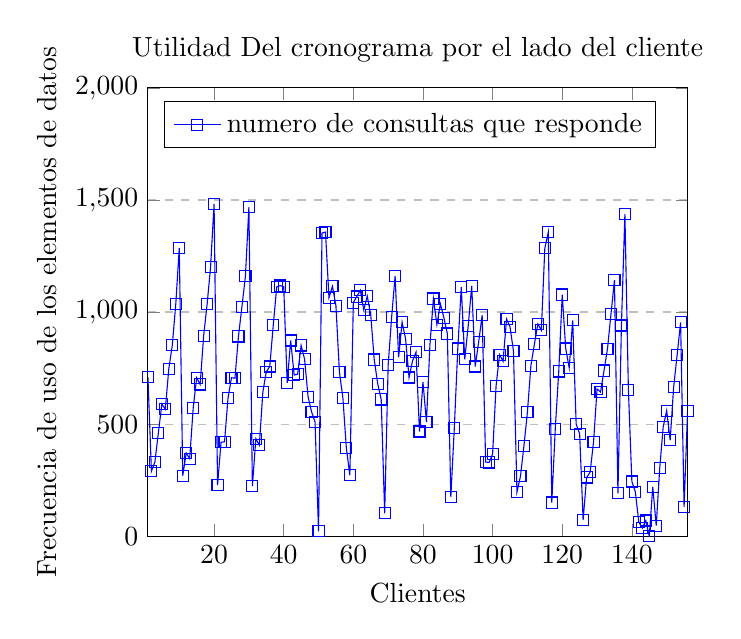
\begin{tikzpicture}
\begin{axis}[
    title={Utilidad Del cronograma por el lado del cliente},
    xlabel={Clientes},
    ylabel={Frecuencia de uso de los elementos de datos},
    xmin=1, xmax=156,
    ymin=0, ymax=2000,
    xtick={},
    ytick={},
    legend pos=north west,
    ymajorgrids=true,
    grid style=dashed,
]

\addplot[
    color=blue,
    mark=square,
    ]
    coordinates {
    %USO EXACTO
    (1,709)
(2,290)
(3,331)
(4,461)
(5,589)
(6,567)
(7,747)
(8,852)
(9,1036)
(10,1286)
(11,270)
(12,371)
(13,346)
(14,571)
(15,707)
(16,677)
(17,893)
(18,1035)
(19,1202)
(20,1482)
(21,228)
(22,419)
(23,421)
(24,616)
(25,707)
(26,705)
(27,891)
(28,1024)
(29,1159)
(30,1469)
(31,223)
(32,435)
(33,406)
(34,642)
(35,734)
(36,757)
(37,942)
(38,1112)
(39,1118)
(40,1113)
(41,684)
(42,873)
(43,719)
(44,722)
(45,851)
(46,789)
(47,622)
(48,555)
(49,510)
(50,22)
(51,1352)
(52,1357)
(53,1064)
(54,1115)
(55,1028)
(56,733)
(57,617)
(58,392)
(59,272)
(60,1042)
(61,1069)
(62,1097)
(63,1009)
(64,1071)
(65,987)
(66,788)
(67,680)
(68,610)
(69,102)
(70,763)
(71,977)
(72,1161)
(73,798)
(74,955)
(75,881)
(76,708)
(77,782)
(78,821)
(79,467)
(80,688)
(81,509)
(82,854)
(83,1060)
(84,944)
(85,1036)
(86,975)
(87,904)
(88,175)
(89,482)
(90,837)
(91,1111)
(92,789)
(93,939)
(94,1117)
(95,757)
(96,867)
(97,986)
(98,331)
(99,329)
(100,366)
(101,671)
(102,810)
(103,780)
(104,969)
(105,934)
(106,825)
(107,197)
(108,267)
(109,403)
(110,553)
(111,761)
(112,856)
(113,947)
(114,919)
(115,1285)
(116,1356)
(117,150)
(118,480)
(119,735)
(120,1078)
(121,837)
(122,751)
(123,963)
(124,500)
(125,457)
(126,72)
(127,262)
(128,285)
(129,421)
(130,657)
(131,643)
(132,739)
(133,836)
(134,991)
(135,1142)
(136,191)
(137,940)
(138,1438)
(139,654)
(140,244)
(141,197)
(142,63)
(143,36)
(144,70)
(145,0)
(146,220)
(147,47)
(148,303)
(149,488)
(150,560)
(151,428)
(152,665)
(153,808)
(154,954)
(155,131)
(156,560)
(157,399)
    };
    \legend{numero de consultas que responde}

\end{axis}
\end{tikzpicture}

